\documentclass[a4paper, twocolumn, 11pt, twoside]{article}

% update your language here.
\usepackage[portuges]{babel}
\usepackage{linguamatica}

% added packages
\usepackage{fancyvrb}
\usepackage{graphicx}
\usepackage{comment}
\usepackage{amsmath}
\usepackage{commath}
\usepackage{makecell} % for formating column heads
\renewcommand\theadfont{\bfseries}
\usepackage{subcaption}	% for \subtable
\usepackage{listings} % see below
\usepackage[]{program}
\usepackage{color}
\usepackage{multirow}


%% Please use UTF8 in your document

%% Set the bibliography style.
%% Styles provided for Spanish (Castilian), Catalan and Portuguese.
%% Other languages will be created on a required basis.

\bibliographystyle{sp_por}   % This for Portuguese


%% You can leave this unchanged. It will be updated by the editors when your paper gets published.
\submitted{15 de \OCT{} 2017}
\accepted{3 de \DEC{} 2017}


%% Add your title in the main language used in the article
\title{Extracção de Relações de Apoio e Oposição \\em Títulos de Notícias de Política}

%% Currenty the title in English is also mandatory
\titleEN{Extraction of Support and Opposition Relationships in Portuguese Political News Headlines}


%% Add authors here. Three lines for each author.
%% First line with author name, second with the affiliation and third with e-mail
%% In cases where a second line is needed for the affiliation, use the command \nl to separate them. 
\author{
  David S. Batista \\
  %\instituto{}
  \email{dsbatista@gmail.com} 
}


\begin{document}
\maketitle

%% Add the abstract in the main language for the article. If possible, doesn't add any citations here.
\begin{resumo}
Os títulos de notícias de política relatam com frequência interacções envolvendo personalidades políticas, sendo que muitas dessas interacções correspondem a relações de apoio ou oposição de uma personalidade para outra, por exemplo: \textit{``Marques Mendes critica estratégia de Rui Rio"} ou \textit{``Costa reafirma confiança em Centeno"}.

Neste trabalho, analisámos centenas de milhares de títulos de notícias de artigos arquivados, identificando aqueles que expressam relações de apoio ou oposição entre duas personalidade políticas. Neste processo também associámos as personalidades políticas com o seu identificador na Wikidata. 

Este processo resultou num grafo semântico onde os nós são personalidades representadas na Wikidata ligadas através de vértices representando relações de oposição ou apoio suportadas por uma notícia. O grafo permite responder a diferentes tipos de interrogações envolvendo personalidades políticas e partidos, e.g.: \textit{Que personalidades do BE se opuseram a personalidades do PCP?}, \textit{Quem do PS apoiou/se opôs a José Sócrates?}, \textit{Que personalidades do PS apoiaram personalidades do PSD?}

Neste artigo descrevemos o processo de extracção dos triplos que compõem o grafo semântico e tornamos acessível uma colecção de dados anotada manualmente. A colecção de dados anotada permitiu treinar classificadores de aprendizagem supervisionada para identificar as relações expressas nos títulos e ligar as personalidades referidas com a Wikidata. 

Tornamos também disponível o grafo resultante do processo de extracção, contendo um total de 680 personalidades políticas e referindo mais de 10 mil notícias, onde existe um sentimento de apoio ou oposição entre duas personalidades políticas, cobrindo um período de 25 anos.

No contexto de análise de notícias de política em Português, e tanto quanto é do nosso conhecimento, este é um trabalho seminal, propondo um método para extrair relações de apoio e oposição entre personalidades políticas.
\end{resumo}

%% Add keywords in the article main language, in lowercase
\palavraschave{extracção de relações semânticas, dados anotados, web semântica, RDF, PLN, ciência política}

%% Add the abstract in English
\begin{abstract}

Political news headlines often report on interactions involving political personalities, many of these interactions correspond to relationships of support or opposition from one personality to another, for example: \textit{``Marques Mendes criticizes Rui Rio's strategy"} or \textit{``Costa reaffirms confidence in Centeno"}

In this work, we analysed hundreds of thousands of archived news titles identifying those that express support or opposition relationships between two political personalities. In this process we also associated the political personalities with their unique identifier in Wikidata. 

This process resulted in a semantic graph where the nodes are personalities represented by Wikidata identifiers and connected through vertices representing opposition or support relationships supported by a news article. The graph allows answering different types of queries involving political personalities and parties, e.g.: \textit{Which BE personalities opposed Jerónimo de Sousa?}, \textit{Which BE personalities opposed PCP personalities?}, \textit{Who from the PS opposed/supported José Sócrates?}, \textit{Which PS personalities have supported PSD personalities?}.

In this paper we describe the process of extracting the semantic triples that make up the semantic graph and we make publicly available a manually annotated dataset. The dataset allowed us to train supervised machine learning classifiers to automatically identify the relationships expressed in the titles and to link the referred personalities to Wikidata. 

We also made publicly available the graph resulting from the extraction process, containing a total of 680 political personalities and referring more than 10,000 news stories covering a period of about 25 years.

In the context of political news analysis in Portuguese, and to the best of our knowledge, this is a seminal work, proposing a method to extract relationships of support and opposition between political personalities.

\end{abstract}

%% add the keywords in English
\keywords{semantic relationship extraction, annotated dataset, semantic web, RDF, NLP, political science}

\section{Introdução}
\label{sec:intro}

Os títulos de notícias relacionados com política ou políticos relatam com frequência interacções envolvendo duas ou mais personalidades políticas. Muitas dessas interacções correspondem a relações de apoio ou oposição de uma personalidade para uma outra personalidade, por exemplo:

\begin{itemize}
\item{\textit{``Marques Mendes critica estratégia de Rui Rio"}}
\item{\textit{``Catarina Martins pede a demissão do governador Carlos Costa"}}
\item{\textit{``Sócrates foi às bases apelar ao voto em Soares"}}
\end{itemize}

A análise de um grande número deste tipo de relações ao longo do tempo permite vários estudos, por exemplo: encontrar quais as grandes comunidades de apoio ou oposição em função dos governos no poder, ou encontrar as grandes alianças e oposições e as suas dinâmicas. Pode-se também explorar individualmente uma personalidade ao longo do tempo, por exemplo, comparando as relações de apoio ou oposição antes de tomar posse em determinado cargo público com as relações depois de ter assumido o cargo, ou ver que relações de apoio subitamente emergiram. Uma base de dados reunindo notícias expressando relações de apoio ou oposição entre personalidades políticas pode ser usada para rapidamente reunir uma colecção de notícias contendo ou envolvendo personalidades e partidos políticos específicos, por exemplo, para auxiliar numa tarefa de jornalismo de investigação. 

Tendo um método automático para extrair relações e podendo aplicá-lo a uma colecção de dados abrangendo longos períodos de tempo permitiria concretizar os exemplos descritos anteriormente.

Neste trabalho apresentamos um método para extrair relações de apoio ou oposição entre personalidades políticas e descrevemos os resultados da aplicação do mesmo a uma colecção de notícias abrangendo um período de cerca de 25 anos. Durante o processo de extracção das relações ligamos as personalidades políticas envolvidas com o seu identificador na Wikidata~\citep{MKGGB2018} enriquecendo assim a relação com informação associada à personalidade (e.g.: afiliação política, cargos públicos exercidos, legislaturas, relações familiares, etc.). 

Todas as relações extraídas são representadas sob a forma de triplos semânticos seguindo a norma Resource Description Framework (RDF)~\citep{schreiber2014primer}. As personalidades políticas envolvidas, representadas pelo seu identificador na Wikidata, são ligadas através de uma relação de oposição ou apoio representada pela notícia que dá suporte à relação. Esta estrutura dá assim origem a um gráfico semântico, sendo então possível formular interrogações SPARQL~\citep{2013sparql} envolvendo a informação da Wikidata associada a cada personalidade e as relações extraídas dos títulos de notícias, por exemplo:

\begin{itemize}
\item{Listar todas as notícias onde a personalidade X se opõe à personalidade Y}
\item{Listar os membros de um determinado partido que apoiaram alguma personalidade específica}
\item{Listar os membros de um determinado partido apoiados/opostos por membros de um outro partido}
\item{Listar personalidades que estão ligadas através de uma relação familiar e de uma relação de oposição/apoio}
\item{Listar personalidades que fazem parte do mesmo Governo e que estão envolvidas numa relação de oposição/apoio}
\end{itemize}

As principais contribuições deste trabalho são: 

\begin{itemize}
\item{um grafo semântico ligando personalidades políticas representadas na Wikidata através de uma relação de oposição ou apoio suportada por uma notícia}
\item{um conjunto de dados anotados utilizado para treinar os classificadores de extracção de relações sentimento direccionado de títulos de notícias, e também para ligar as personalidades mencionadas à Wikidata}
\item{um interface web que permite explorar o gráfico semântico}
\end{itemize}

Este artigo está organizado da seguinte forma: na Secção~\ref{sec_related_work} referimos trabalho relacionado, na Secção~\ref{sec_kb} descrevemos a base de conhecimento usada no suporte de ligação das personalidades políticas à Wikidata. A Secção~\ref{sec:data_sources} refere e descreve as fontes de notícias utilizadas. Na Secção~\ref{sec:rel_data_annot} detalhamos o conjunto de dados anotados e na Secção~\ref{sec:classifiers} os classificadores de aprendizagem supervisionada desenvolvidos. Na Secção~\ref{sec:pipeline} descrevemos o processo de extracção de triplos RDF e a construção do gráfico semântico. Finalmente, na Secção~\ref{sec:future_work} apresentamos ideias futuras para melhorar e continuar este trabalho.

\section{Trabalho Relacionado}
\label{sec_related_work}
A análise de sentimento, no contexto de Processamento de Linguagem Natural, tem sido maioritariamente alvo de estudo em conteúdo gerado em redes sociais~\citep{10.1145/3185045} ou na avaliação de produtos ou serviços~\citep{pontiki-etal-2016-semeval}. Nestes domínios o autor do texto e o alvo da opinião são explícitos. No contexto de análise de notícias de política, onde existe com frequência um sentimento expresso entre actores políticos sob a forma de relações de apoio ou oposição~\citep{balahur2009opinion, balahur-etal-2010-sentiment}, as abordagens de análise de sentimento a produtos ou serviços não se aplicam, dado que a direcção da relação de sentimento tem que ser considerada.

Nesta secção descrevemos recursos semelhantes aos que produzimos neste trabalho, que tornamos públicos, e abordagens para a tarefa de extracção de sentimento direccionado em texto de notícias de política.

\subsection{Recursos e dados anotados}

% Datasets
% 2009 - https://dl.acm.org/doi/abs/10.1145/1651461.1651468 - Automatic creation of a reference corpus for political opinion mining in user-generated content
% 2013 - http://www.emeraldinsight.com/doi/abs/10.1108/00330331311313708 -  Tracking politics with POWER
% 2015 - https://aclanthology.org/W15-5614/ - An Annotated Corpus for Sentiment Analysis in Political News
% 2021 - https://www.sciencedirect.com/science/article/pii/S1877050921018755 - A dataset for Sentiment analysis of Entities in News headlines (SEN)

\cite{10.1145/1651461.1651468} propõem um método para a criação automática de um corpus para detecção de um sentimento positivo ou negativa para com uma personalidade política, e aplicam o método a comentários a notícias de jornais \textit{on-line}. Neste recurso a origem do sentimento, pressupõem-se, é do comentador.

\cite{moreira2013tracking} disponibilizam uma ontologia descrevendo actores políticos, os seus cargos e partidos políticos afiliados, usando fontes de informação oficiais e informação recolhida da \textit{web} para adicionar nomes alternativos às personalidades presentes na ontologia.

\cite{de-arruda-etal-2015-annotated} criaram um corpus de notícias políticas em português do Brasil, anotando cada parágrafo com o sentimento segundo duas dimensões: o actor político referido pelo parágrafo, e o sentimento dessa referência: positivo, negativo ou neutro. Neste recurso fica em aberto qual é a origem do sentimento. \cite{BARANIAK20213627} disponibilizam corpora semelhante, anotando o sentimento para com uma personalidade política em textos de jornais \textit{on-line}, para o Inglês e Polaco.

\subsection{Extracção de sentimento direccionado em texto de notícias}

Vários autores exploraram métodos para extrair sentimento envolvendo actores político. De notar que muitos dos trabalhos transformam a tarefa de detecção de sentimento numa tarefa de detecção de uma relação entre entidades mencionadas~\citep{bassignana-plank-2022-mean}.

% 2013 - https://aclanthology.org/P13-1108.pdf Learning to Extract International Relations from Political Context
% 2019 - https://aclanthology.org/N19-1167.pdf No Permanent Friends or Enemies: Tracking Relationships between Nations from News
Alguns exploram estas relações num contexto de política internacional, i.e.: os actores são nações referidas em texto de notícias de política, sendo que algumas dessas relações implicitamente têm um sentimento positivo ou negativo. \cite{oconnor-etal-2013-learning} propõem um modelo não supervisionado baseado em \textit{topic models} e padrões linguísticos para identificar relações, de forma aberta, descrevendo conflitos entre nações referenciadas em artigos de notícias em Inglês. \cite{han-etal-2019-permanent} propõem também um modelo não supervisionado para gerar descritores de relações para pares de nações mencionadas em notícias em Inglês.
O modelo proposto estende o trabalho de \cite{iyyer-etal-2016-feuding} integrando informação linguística (i.e.: predicados verbais e substantivos comuns e próprios) por forma a identificar o contexto das relações.

% 2019
% Who Blames Whom in a Crisis? Detecting Blame Ties from News Articles Using Neural Networks 
% https://ojs.aaai.org/index.php/AAAI/article/view/3842/3720
\cite{liang2019blames} define a tarefa de extracção de relações de culpabilidade para textos em inglês: dado um artigo $d$ e um conjunto de entidades $E$, presentes no artigo, detectar se existe uma relação de culpabilidade $(s,t)$, onde $s,t \in E$, quando $s$ culpa $t$ com base no artigo $d$, sendo que há $\lvert{E}\rvert \cdot (\lvert{E}\rvert - 1)$, possíveis relações de culpabilidade. Para detectar estas relações os autores propõem 3 modelos. O modelo \textit{Entity Prior} extrai informação sobre entidades, tentando capturar um \textit{prior} sobre quem é susceptível de culpar quem sem informação adicional. O modelo \textit{Context} faz uso da informação de contexto da frase onde duas entidades ocorrem para determinar a presença de uma relação de culpabilidade. Finalmente o modelo \textit{Combined} combina informação recolhida pelos dois modelos anteriores num único modelo. Os autores aplicam esta abordagem num corpus com 998 artigos de notícias em Inglês com cerca de 3 entidades por artigo e reportam uma macro-média F\textsubscript{1} de 0,70 com o modelo \textit{Combined}.

% 2021
% Who Blames or Endorses Whom? Entity-to-Entity Directed Sentiment Extraction in News Text
% https://aclanthology.org/2021.findings-acl.358/
\cite{park-etal-2021-blames} propõe uma estrutura de relações para detectar o sentimento e a direcção: dada uma frase $s$ referindo duas entidades $p$ e $q$, detectar qual a relação de sentimento entre $p$ e $q$ de entre cinco possíveis: neutra, $p$ tem uma opinião positiva ou negativa em relação a $q$, ou $q$ tem uma opinião positiva ou negativa em relação a $p$. No seu trabalho os autores usam múltiplos modelos transformando a tarefa de extracção de sentimentos em sub-tarefas que respondem a perguntas de sim/não para cada um dos 5 sentimentos possíveis, combinando depois os vários resultados num resultado final. Esta abordagem é aplicada para Inglês num corpus criado pelos autores contendo frases de artigos de notícias contento pelo menos duas entidades, e anotado duas entidades. Os pares de entidades estão anotadas com um dos 5 sentimentos possíveis. Os autores reportam uma macro-média de F\textsubscript{1} de 0,68.

\begin{table*}[!h]
  \centering
  \begin{tabular}{lc}
      {\bf Título} & {\bf Relação} \\
      \hline
	  \textbf{Sá Fernandes} acusa \textbf{António Costa} de defender interesses corporativos &	Ent\textsubscript{1}-opõe-se-Ent\textsubscript{2} \\
	  \textbf{Joana Mortágua}: declarações de \textbf{Cavaco} são ``uma série de disparates" & Ent\textsubscript{1}-opõe-se-Ent\textsubscript{2} \\
	  \textbf{Passos Coelho} é acusado de imaturidade política por \textbf{Santos Silva} &	Ent\textsubscript{2}-opõe-se-Ent\textsubscript{1}	\\
	  \textbf{Durão Barroso} defende \textbf{Paulo Portas} como ``excelente ministro" & Ent\textsubscript{1}-apoia-Ent\textsubscript{2}	\\
	  \textbf{Armando Vara} escolhido por \textbf{Guterres} para coordenar autárquicas & Ent\textsubscript{2}-apoia-Ent\textsubscript{1}	\\
	  \textbf{Manuel Alegre} recebe apoio de \textbf{Jorge Sampaio} & Ent\textsubscript{2}-apoia-Ent\textsubscript{1}	\\
	  \textbf{Rui Tavares} e \textbf{Ana Drago} eleitos nas primárias do LIVRE & outra	\\
	  \textbf{Teresa Zambujo} reconhece vitória de \textbf{Isaltino Morais} & outra	\\
	  CDS acusa \textbf{Marcelo Rebelo de Sousa} de pôr em causa relação com \textbf{Cavaco} & outra \\
	  \hline
  \end{tabular}
  \caption{Exemplos de títulos e das relações manualmente anotadas correspondentes.}
  \label{tab:samples}
\end{table*}

\section{Base de Conhecimento}
\label{sec_kb}
Dado que as personalidades envolvidas nas relações a extrair são personalidades políticas relevantes, começámos por construir uma base de conhecimento a partir da Wikidata~\citep{MKGGB2018}. Fazendo interrogações SPARQL ao \textit{endpoint} público\footnote{\url{https://query.wikidata.org}} recolhemos o identificador de todas as:

\begin{itemize}  
\item pessoas que são ou foram afiliadas a algum partido político português
\item pessoas portuguesas nascidas depois de 1935 cuja profissão seja: \textit{juiz, economista, advogado, funcionário público, político, empresário ou banqueiro}
\item pessoas que têm ou tiveram pelo menos um cargo de uma lista de cargos públicos portugueses previamente seleccionados (e.g.: \textit{ministro, líder do partido, embaixador}, etc.)
\end{itemize}  

Para além dos resultados destas interrogações, seleccionámos manualmente alguns identificadores de personalidades não abrangidas pelas interrogações SPARQL definidas acima, muitas delas de um contexto político internacional, mas que interagem com personalidades portuguesas. Acrescentámos também todos os identificadores de partidos políticos a que as personalidades recolhidas estão afiliadas. Este processo resultou num total de 1 757 personalidades e de 37 partidos políticos. De notar que alguns dos partidos incluídos são partidos já extintos e/ou de um contexto internacional. Para cada um dos identificadores das personalidades e partidos descarregamos a página correspondente na Wikidata utilizando um outro \textit{endpoint}\footnote{\url{https://www.wikidata.org/wiki/Special:EntityData?}} público.

% SELECT (COUNT(DISTINCT ?person) as ?nr_persons) {?person wdt:P31 wd:Q5;}
% SELECT (COUNT(DISTINCT ?person) as ?nr_parties) {?person wdt:P31 wd:Q7278;}

Para cada personalidade política seleccionámos: o seu identificador na Wikidata, o seu nome mais comum e os nomes alternativos, i.e.: combinações de nomes próprios e apelidos. Com base nestes três campos, criámos um índice no ElasticSearch~\citep{10.5555/2904394} usando a sua configuração de omissão, não fazendo uso de qualquer funcionalidade extra tais como analisadores de $n$-gramas.

\section{Fontes de dados}
\label{sec:data_sources}

A principal fonte de notícias foi o arquivo da \textit{web} portuguesa~\citep{SearchPastPWA2013}. Usando a API pública de pesquisa recolhemos páginas arquivadas restringindo os resultados a ocorrências de nomes reunidos na Secção~\ref{sec_kb} e a 45 domínios \texttt{.pt} associados a diversas fontes de informação: jornais \textit{on-line}, \textit{websites} de estações de televisão e rádio, e portais agregadores de conteúdos. 

Uma segunda fonte de notícias foi a colecção CHAVE\footnote{\url{https://www.linguateca.pt/CHAVE/}}\citep{DBLP:conf/clef/SantosR04, santos-rocha-2001-evaluating}, contendo os artigos do jornal PÚBLICO publicados entre 1994 e 1995. Finalmente, foram também adicionados alguns artigos não arquivados pelo arquivo.pt, retirados directamente das secções {\it Mundo}, {\it Política} e {\it Sociedade} do site publico.pt. 

Deste processo resultou uma colecção de cerca de 13,7 milhões de títulos de artigos publicados entre 1994 e 2022. De seguida foi aplicado um pré-processamento de modo a remover notícias com: títulos duplicados, títulos com menos de 4 palavras, e títulos ou URLs contendo palavras que fazem partem de uma lista pré-definida (e.g.: \textit{desporto}, \textit{celebridades}, \textit{artes}, \textit{cinema}, etc.) que sugerem um o outro contexto que não política. Este pré-processamento resultou em 1,3 milhões de títulos distintos, cerca de 10\% dos dados inicialmente recolhidos.

\section{Colecção de Relações Anotadas}
\label{sec:rel_data_annot}

De forma a poder treinar classificadores de aprendizagem supervisionada para identificar as relações presentes nos títulos das notícias, e fazer a ligação das personalidades com a Wikidata, anotámos manualmente títulos com: as menções a personalidades, os identificadores na Wikidata e a relação entre as personalidades mencionadas.

Começámos por pré-processar todos os títulos recolhidos usando o pacote de software spaCy 3.0~\citep{spacy}, com o modelo~\texttt{pt\_core\_news\_lg-3.0.0} fizemos o reconhecimento de entidades mencionadas do tipo \texttt{PESSOA}. Para cada entidade reconhecida tentamos encontrar o seu identificador correspondente na Wikidata fazendo uma interrogação ao índice descrito na Secção~\ref{sec_kb} e assumindo que na lista de resultados o primeiro é o identificador correcto associado à entidade. Seleccionamos depois os títulos para anotação, incluindo apenas títulos referindo pelos menos duas personalidades.

No processo de anotação todos os títulos foram carregados para ferramenta de anotação Argilla\footnote{\url{https://github.com/argilla-io/argilla}}, e usando o interface gráfico fomos selecionando títulos para anotar. 

Para cada título corrigimos sempre que necessário as entidades reconhecidas e os seus identificadores na Wikidata, caso existam. Anotámos a relação existente: \textbf{oposição} ou \textbf{apoio}, e a direcção da mesma. Quando nenhuma das duas se verifica a relação é anotada como \textbf{outra}. A Tabela~\ref{tab:samples} demonstra alguns exemplos das relações anotadas. O processo de anotação foi feito por um anotador. Nas situações mais ambíguas, por exemplo, onde é necessária a informação no texto da notícia para decidir, as relações foram anotados como \textbf{outra}.

Este processo resultou num conjunto de dados contendo 3.324 títulos anotados. Para cada título anotámos apenas duas personalidades e a relação entre elas, mesmo que os títulos contenham referências a mais do que duas personalidades. A Tabela~\ref{tab:rel_dataset} caracteriza os dados em termos de número de relações e direcção. A maioria dos títulos contém uma relação de \textbf{oposição} ou \textbf{outra}, e a grande maioria das relações têm uma direcção da primeira para a segunda entidade, Ent\textsubscript{1}$\rightarrow$Ent\textsubscript{2}.

% jq -r '"\(.label)"' < politiquices_data_v3.0.jsonl | sort | uniq -c

\begin{table}[!h]
    \begin{center}
    \begin{tabular}{l ccr}
        {\bf Relação} & {\bf \footnotesize{Ent\textsubscript{1}$\rightarrow$Ent\textsubscript{2}}} & {\bf \footnotesize{Ent\textsubscript{1}$\leftarrow$Ent\textsubscript{2}}} & {\bf Total} \\
        \hline
        opõe-se          &  1 155  &  102  &  1 257  \\
        apoia            &    717  &   44  &    761  \\
        outra            &    -    &   -   &  1 306  \\
		\hline
		Total			 &  1 872  &  146  &  3 324  \\
    \end{tabular}
	\caption{Relações por classe e direcção.}
	\label{tab:rel_dataset}
	\end{center}
\end{table}

O rácio de relações de oposição para com relações de apoio é de 1,6, este valor é semelhante com os dados para Inglês disponibilizados por~\cite{park-etal-2021-blames}, onde esta mesma relação entre as duas classes é de 1,8.  Em termos de representatividade das classes, agregadas por sentimento, os dois conjuntos de dados também são semelhantes, sendo \textbf{outra} a classe mais presente, seguindo-se \textbf{oposição} e por último \textbf{apoio}.

% fazer uma comparação com este dataset
% Negative:  3,163 + 478 ->  3 641 -> 22%
% Positive:  1,656 + 327 ->  1 983 -> 12%
% Neutral : 10,604	     -> 10 604 -> 65%

% Negative (p → q) 3,163
% Positive (p → q) 1,656 
% Positive (p ← q) 327
% Negative (p ← q) 478

% p → q -> 4819  (29%)
% p ← q -> 805   (5%)
% Neutral 10,604 (65%)
% 16.228

% jq -r '"\(.ent1_id) \(.ent2_id)"' < politiquices_data_v3.0.jsonl | tr ' ' '\n' | sort | uniq -c | sort -gr

\begin{figure}
  \centering
    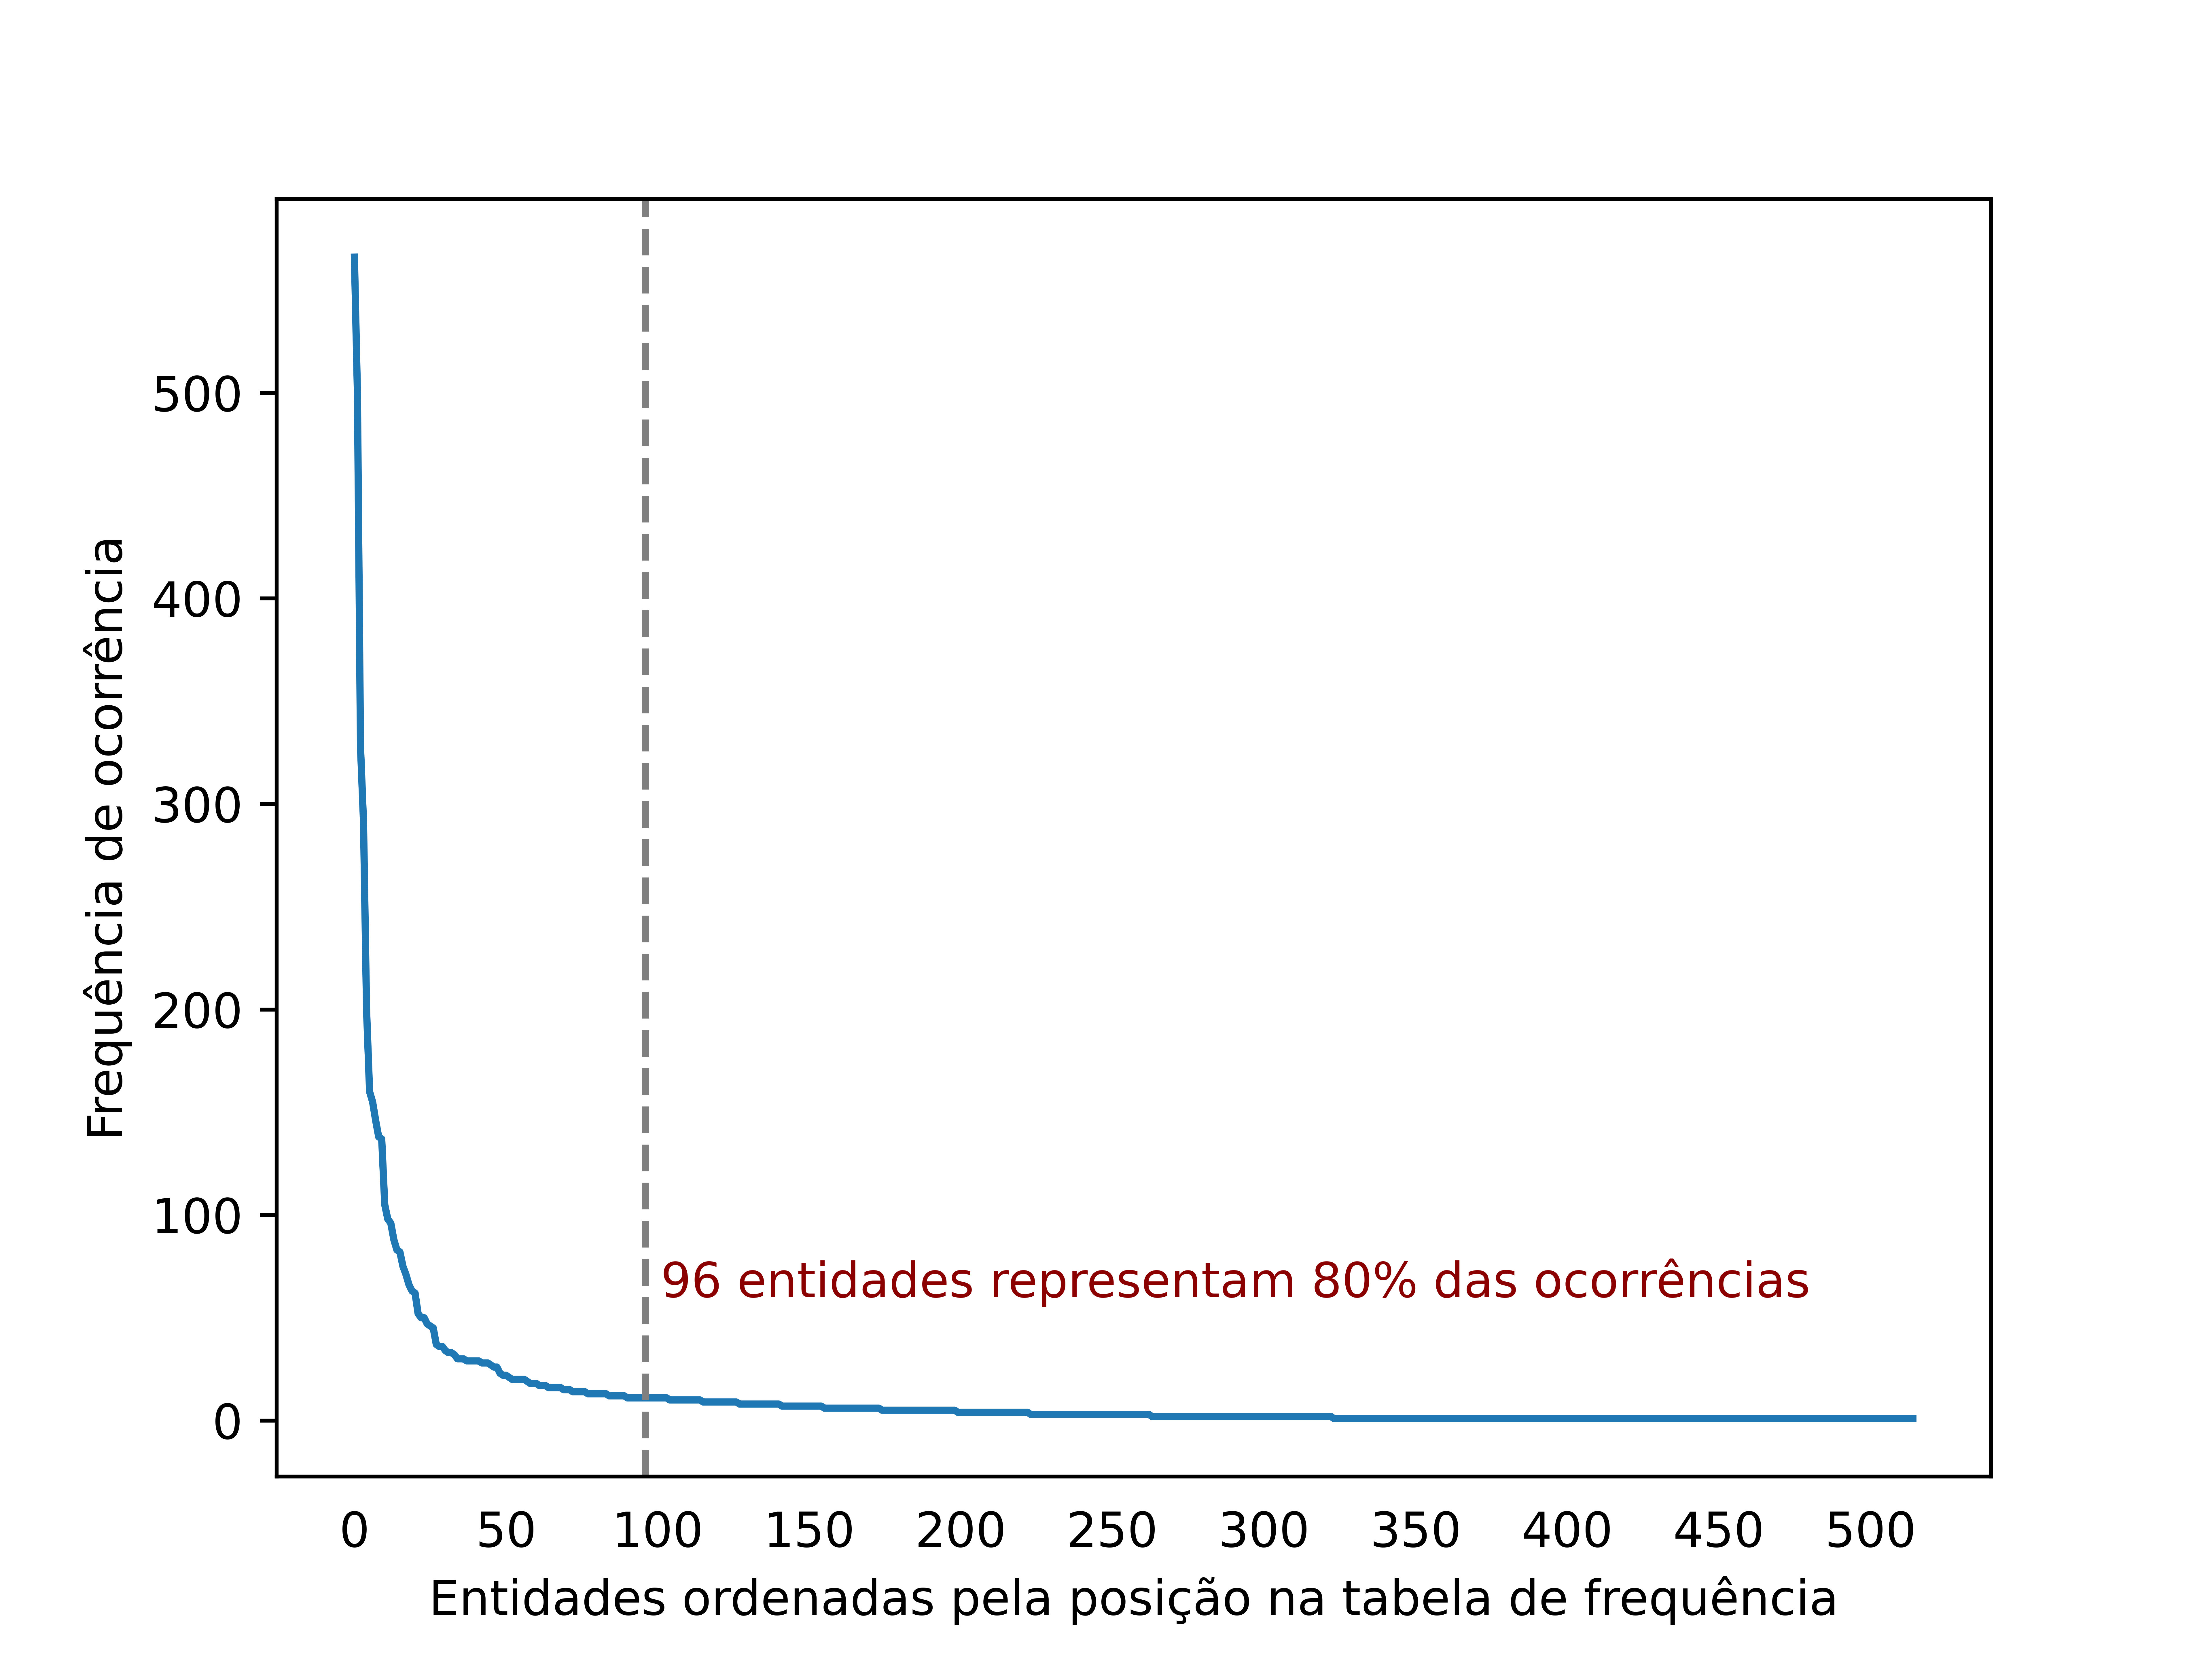
\includegraphics[width=0.53\textwidth]{power_law_ent_freq.png}
  \caption{Distribuição de frequências de ocorrências das personalidades nos títulos anotados.}
  \label{fig:ent_power_law}
\end{figure}

Das 6.648 menções a nomes de personalidades políticas anotadas, 515 são distintas e têm um identificador na Wikidata. Um total de 129 entidades distintas, identificadas por agregação da \textit{string} que as refere no título, não estão associadas a um identificador por não estarem presentes na Wikidata. 

Analisando a frequência de ocorrência de cada entidade observa-se que há pequeno número de entidades responsáveis por uma grande parte de todas as ocorrências de entidades nos dados anotados. Como mostra a Figura~\ref{fig:ent_power_law} existe um número pequeno de entidades frequentes, e uma longa lista de entidades pouco frequentes, em concreto, 96 personalidades distintas, i,.e.: 19\% das personalidades, são responsáveis por 80\% das menções a personalidades nos dados.

Em termos de número de palavras contidas no título, excluindo palavras que fazem parte das entidades envolvidas numa relação, têm um mediana de 8 palavras com um máximo de 22 e um mínimo de 1. Este conjunto de dados anotados encontram-se online\footnote{\url{https://github.com/politiquices/data-releases}} sob o formato JSON como ilustrado na Figura~\ref{fig:json_sample}.

\begin{figure}[!h]
\begin{Verbatim}[fontsize=\small]
  {"title": "Ana Gomes defende Durão Barroso",
   "label": "ent1_supports_ent2",
   "date": "2002-05-11 08:26:00",
   "url": "http://www.publico.pt/141932",
   "ent1": "Ana Gomes",
   "ent2": "Durão Barroso",
   "ent1_id": "Q2844986'",
   "ent2_id": "Q15849"}
\end{Verbatim}
  \caption{Exemplo de um título anotado sob o formato JSON.}
  \label{fig:json_sample}
\end{figure}

\section{Processo de Extracção de Relações}
\label{sec:classifiers}

O processo de extração de triplos RDF a partir dos títulos das notícias envolve 4 sub-processos:

\begin{itemize}
\item reconhecimento de entidades-mencionadas do tipo \texttt{PESSOA}
\item ligação das entidades com um identificador na Wikidata
\item classificação do tipo de relação
\item classificação da direcção da relação
\end{itemize}

\subsection{Reconhecimento de Entidades}
\label{subsec:ner}

% https://spacy.io/usage/rule-based-matching

O reconhecimento de entidades mencionadas é baseado num método híbrido, combinando regras com um modelo supervisionado.

Usando a componente \texttt{EntityRuler}\footnote{\url{https://spacy.io/usage/rule-based-matching}} do spaCy 3.0, definimos uma série de regras combinando padrões baseados nos nomes de todas as personalidades da base de conhecimento descrita na Secção~\ref{sec_kb}. Para detectar as entidades do tipo \texttt{PESSOA} este classificador aplica primeiro as regras e de seguida o modelo supervisionado para Português do spaCy. Em situações de desacordo entre as duas abordagens as entidades marcadas com regras têm prioridade.

A Tabela~\ref{tab:results_ner} mostra a performance para as 3 abordagens sob o conjunto de dados anotado.

% jq -r '"\(.ent1)|\(.ent2)"' < politiquices_data_v3.0.jsonl | tr '|' '\n' | wc -l

\begin{table}[!h]
    \begin{center}
    \begin{tabular}{l ccc}
		{\bf Abordagem}  & {\bf P} & {\bf A} & {\bf F\textsubscript{1}} \\
        \hline
        Regras           &  0,99     &  0,42     & 		0,59		\\
        Modelo           &  0,97     &  0,91     & 		0,94		\\
		Regras+Modelo    &  0,97     &  0,92     & 		0,94		\\
    \end{tabular}
	\caption{ (P)recisão, A(brangência) e F\textsubscript{1} para a componente de REM combinando regras e o modelos supervisionado.}	
	\label{tab:results_ner}
	\end{center}
\end{table}

\subsection{Ligação com a Wikidata}
\label{subsec:ent_linking}

O algoritmo para associar personalidades com identificadores na Wikidata tem duas fases. Numa primeira fase o algoritmo tenta apenas usar o título da notícia, se este processo falhar, tenta então usar possíveis referências às personalidades no texto da notícia.

O algoritmo começar primeiro por fazer uma interrogação à base de conhecimento (BC), usando a referência à personalidade presente no título, gerando assim uma lista de candidatos para uma determinada personalidade. Se a lista contém apenas um candidato e a similaridade~\citep{jaro1989} para com a personalidade referida no título é de pelo menos 0,8 esse candidato é seleccionado. Se houver mais do que um candidato, o algoritmo filtra apenas aqueles com uma similaridade de 1,0 e se houver apenas um esse é o candidato seleccionado. Em qualquer outro caso nenhum candidato é retornado. 

O Algoritmo 1 descreve o procedimento que usa apenas o título da notícia.

\begin{lstlisting}[language=python,columns=fullflexible,frame=single,label={lst:alg1},title={Algoritmo 1. Ligação com a Wikidata usando apenas o título.},captionpos=b]
def title_only(ent, candidates):
    if len(candidates) == 1:
      if jaro(ent,candidates[0]) >= 0.8:
        return candidates[0]
    else:
      filtered = exact(ent, candidates):
	if len(filtered) == 1:
	  return candidates[0]
    return None
\end{lstlisting}

Se nenhum candidato for gerado na primeira fase ou nenhum for seleccionado da lista de candidatos o algoritmo tenta expandir as entidades mencionadas no título com base no texto da notícia, explorando um padrão: uma personalidade mencionada no título por uma versão curta do seu nome, e.g.: apenas o apelido, é normalmente referida no texto da notícia por um nome mais completo.

O algoritmo identifica todas as pessoas mencionadas no texto da notícia, usando a componente descrita na Secção~\ref{subsec:ner}, e seleciona apenas as que têm pelo menos um nome em comum com o nome da personalidade referida no título, gerando assim uma entidade expandida, e assumindo que corresponde à mesma entidade referida no título.

Se do processo resulta apenas uma entidade expandida e se há uma similaridade de 1.0 com um dos candidatos anteriormente seleccionados da BC, esse candidato é escolhido. Caso contrário a entidade expandida é usada para fazer uma interrogação à BC e recolher uma nova lista de candidatos. Se nessa lista apenas há um candidato e a sua similaridade é de pelo menos 0.8 para com a entidade expandida, esse candidato é escolhido. Se há mais do que um candidato e apenas um tem uma similaridade 1.0 com a entidade expandida, esse é escolhido. 

Se do processo de expansão resultam várias entidades expandidas, filtramos candidatos da BC com similaridade 1.0 para com a entidade expandida, se existir apenas um, esse candidato é o escolhido. 

Em qualquer outro caso aqui não descrito nenhum candidato é selecionado.

O Algoritmo 2 descreve este procedimento usando o texto da notícia.

\begin{lstlisting}[language=python,columns=fullflexible,frame=single,label={lst:alg2},title={Algoritmo 2. Ligação com a Wikidata usando o texto da notícia para expandir as entidades reconhecidas no título.},captionpos=b]]
def article_text(expanded, candidates):
  if len(expanded) == 1:
    filtered = exact(expanded[0], candidates)
	if len(filtered) == 1:
	  return filtered[0]
	  
    x_candidates = get_candidates(expanded)
    if len(x_candidates) == 1:
      if jaro(expanded, x_candidates[0])>=0.8:
        return x_candidates[0]
 
    filtered = exact(expanded, x_candidates)
    if len(filtered) == 1:
      return matches[0]
  
  if len(expanded) > 1:
    filtered = []
    for e in expanded:
      exact_candidates = exact(e, candidates)
	  for c in exact_candidates:
	    filtered.append(c)
    if len(filtered) == 1:
      return filtered[0]

  return None
\end{lstlisting}

Os resultados desta abordagem sobre o conjunto de dados anotados são descritos na Tabela~\ref{tab:ent_linking_results}. A classificação \textit{incorrecta} corresponde a personalidades que não foram associadas ao identificador correcto na Wikidata, \textit{não desambiguada} para as que o algoritmo não conseguiu seleccionar um identificador único de entre todos os candidatos ou a BC não retornou nenhum resultado.

Na Tabela~\ref{tab:ent_linking_results} são reportadas duas avaliações, a primeira coluna descreve os resultados para o algoritmo base, sem mapeamentos. A segunda coluna considera a ambiguidade que uma referência pode ter em termos de personalidades que representa. Por exemplo, nos dados anotados, todas as menções a \textit{Cavaco} correspondem à personalidade \textit{Cavaco Silva}, com base nisto o algoritmo mapeia todas as referências a \textit{Cavaco} para \textit{Cavaco Silva}. Da mesma forma, todas as menções a \textit{Marques Mendes} correspondem à personalidade \textit{Luís Marques Mendes}. Fazendo uso destes mapeamentos reduzimos o número de entidades para as quais o algoritmo não consegue encontrar um identificador.

\begin{table}[!h]
    \begin{center}
    \begin{tabular}{l rr}
        {\bf Classificação} & {\bf base} & \it{{\bf mapeamentos}} \\
        \hline
        correcta            &   5 059    &  5 136   \\
        incorrecta          &      43    &     43   \\
		não desambiguada    &     246    &    169   \\    
        \hline
		{\bf Exactidão }    &    0,93	 &  0,96   \\
    \end{tabular}
	\caption{Resultados da avaliação do algoritmo de ligação com a Base de Conhecimento.}
	\label{tab:ent_linking_results}
	\end{center}
\end{table}

\subsection{Classificador de Tipo de Relação}
\label{subsec:rel_classifier}

Optamos por decompor a tarefa de classificação da relação em duas tarefas: classificação do tipo de relação e direcção da relação, por oposição a desenvolver um único classificador que teria que distinguir de entre 5 classes possíveis, e com classes muito desequilibradas em termos de representatividade. Esta secção descreve o classificador desenvolvido para detectar o tipo de relação presente num título, tendo 3 classes possíveis: \textbf{opõe-se}, \textbf{apoia} e \textbf{outra}. Todas as experiências descritas foram feitas com uma avaliação cruzada de 4 partições\footnote{\url{https://github.com/politiquices/data-releases}}.

Avaliámos diferentes abordagens para a classificação supervisionada das relações presentes nos títulos, nomeadamente: um classificador SVM~\citep{cortes1995support} com um \textit{kernel} linear, uma rede neuronal recorrente do tipo LSTM~\citep{10.1162/neco.1997.9.8.1735}, e uma rede neuronal do tipo \textit{transformer}, o DistilBERT~\citep{9463516}.

Para o classificador SVM utilizámos como \textit{features} uma abordagem baseada em vectores TF-IDF~\citep{DBLP:journals/ipm/SaltonB88}, fazendo um pré-processamento do título, usando um padrão, de modo a identificar o contexto relevante, i.e.: o contexto no título que contém informação que descreve a relação: \texttt{<Ent\textsubscript{1} X Ent\textsubscript{2} \textbf{contexto}>} onde \texttt{X} = \{\textit{“diz a”, “responde a”, “sugere a”, “diz que, “afirma que”, “espera que”, “defende que”, “considera que”, “sugere que”, “quer saber se”, “considera”, “manda”}\}. Sempre que o padrão não se verifica usamos todas as palavras do título para construir o vector, excepto o nome das personalidades.

A rede neuronal recorrente LSTM foi usada numa arquitectura bidireccional, ou seja, são usadas duas redes LSTM, ambas com uma dimensão de 128, uma lendo o título da primeira para a última palavra e outra da última para a primeira palavra, sendo que os dois estados finais de cada LSTM são concatenados e passados a um \textit{layer} linear. Usamos \textit{embeddings} pré-treinados para Português baseados no método FastText (\textit{skip-gram}) de dimensão 50~\citep{hartmann-etal-2017-portuguese}. A rede foi treinada por 5 \textit{epochs} com um \textit{batch size} de 8.
%optimizer = optim.Adam(model.parameters())
%criterion = nn.BCELoss()

O modelo DistilBERT foi treinado tendo como base um modelo pré-treinado para o Português~\citep{abdaoui-etal-2020-load}, sendo depois afinado no conjunto de dados anotado, i.e.: os pesos de todos os \textit{layers} pré-treinados foram actualizados tendo em conta a tarefa de classificação da relação. A rede foi treinada durante 5 \textit{epochs} com um \textit{batch size} de 8.
%optimizer = optim.Adam(model.parameters())
%tipo de loss function? nn.BCEWithLogitsLoss(pos_weight=self._class_weights)


\begin{table}
    \begin{subtable}[c]{.5\textwidth}
    \centering
    \begin{tabular}{l ccc}
        {\bf Relação} & {\bf P} & {\bf A} & {\bf F\textsubscript{1}} \\
		\hline
        opõe-se          &  0,71  &  0,69  &  0,70   \\
        outra            &  0,69  &  0,69  &  0,69   \\
        apoia            &  0,65  &  0,69  &  0,67   \\
		\hline
		Macro-Média      &	0,69  &  0,69  &  0,69   \\
    \end{tabular}
    \caption{SVM com um kernel linear.\label{tbl:svmlinearaccuracy}}
    \vspace{5mm}           
    \end{subtable}
\quad%
    \begin{subtable}[c]{.5\textwidth}
    \centering
    \begin{tabular}{l ccc}
        {\bf Relação} & {\bf P} & {\bf A} & {\bf F\textsubscript{1}} \\
		\hline
        opõe-se          &  0,75  &  0,64  &  0,69   \\
        outra            &  0,65  &  0,75  &  0,70   \\
        apoia            &  0,65  &  0,62  &  0,63   \\
		\hline
		Macro-Média      &  0,69  &  0,68  &  0,68   \\
    \end{tabular}
    \caption{LSTM bidireccional.\label{tbl:bilstm}}
    \vspace{5mm}     
    \end{subtable}
\quad%
    \begin{subtable}[c]{.5\textwidth}
    \centering
    \begin{tabular}{l ccc}
        {\bf Relação} & {\bf P} & {\bf A} & {\bf F\textsubscript{1}} \\
		\hline
        opõe-se          &  0,74  &  0,76  &  0,75   \\
        outra            &  0,72  &  0,71  &  0,72   \\
        apoia            &  0,72  &  0,71  &  0,71   \\
		\hline
		Macro-Média      &  0,73  &  0,72  &  0,72   \\
    \end{tabular}
    \caption{DistilBERT pré-treinado em Português.\label{tbl:distilbert}}
    \end{subtable}
  \caption{(P)recisão, (A)brangência e F\textsubscript{1} para uma avaliação com 4-partições e validação cruzada com diferentes classificadores.}
  \label{tab:results_relacao}
\end{table}

A Tabela~\ref{tab:results_relacao} descreve os resultados para os vários classificadores. Não há diferenças muito acentuadas em termos de performance entre os 3 classificadores, embora a abordagem usando o DistilBERT tenha alcançado os melhores resultados. Ao analisar os resultados notamos que há relações difíceis de classificar correctamente, nomeadamente as que contêm expressões idiomáticas, por exemplo:

\begin{itemize}
\item{\textit{José Lello diz que Nogueira Leite quer “abifar uns tachos”}}
\item{\textit{Louçã diz que “António Borges é o grilo falante” de Passo Coelho}}
%\item{\textit{Louçã acusa Passos de ser o “cangalheiro da melhor maternidade” do país}}
\end{itemize}

Outras relações são ambíguas e difíceis de classificar sem mais contexto do que aquele presente no título. No conjunto de dados que tornamos público, todos os títulos contêm um URL para o texto da notícia. 

Os resultados obtidos com as abordagens descritas, para os dados em Português, estão em linha com os resultados reportados anteriormente em dados em Inglês~\citep{liang2019blames, park-etal-2021-blames}.


\begin{table*}
  \centering
  \begin{tabular}{lc}
      {\bf Título} & {\bf Regra Aplicada} \\
      \hline
	  \textbf{Marques Júnior} elogiado por \textbf{Cavaco Silva} pela ``integridade de carácter" & VOZ\_PASSIVA \\
	  \textbf{Passos Coelho} é acusado de imaturidade política por \textbf{Santos Silva}  		 & VOZ\_PASSIVA \\
	  \textbf{António Costa} vive no ``país das maravilhas" acusa \textbf{Assunção Cristas}      & VERBO\_ENT2 \\
	  \textbf{Passos Coelho} ``insultou 500 mil portugueses", acusa \textbf{José Sócrates}		 & VERBO\_ENT2 \\ 
	  \textbf{Maria Luís Albuquerque} sob críticas de \textbf{Luís Amado}						 & NOUN\_ENT2 \\
	  \textbf{André Ventura} diz-se surpreendido com perda de apoio de \textbf{Cristas}			 & NOUN\_ENT2 \\

	  \hline
  \end{tabular}
  \caption{Exemplos de títulos e respectivas regras usadas para detectar a direcção da relação.}
  \label{tab:examples_patterns_direction}
\end{table*}

\subsection{Classificador de Direção da Relação}
\label{subsec:rel_direction}

O classificador da direcção tem 2 classes possíveis. Como mostra a Tabela~\ref{tab:rel_dataset}, o conjunto de dados tem um viés para com a classe Ent\textsubscript{1}$\rightarrow$Ent\textsubscript{2} representando 91,5\% dos dados. Assim, optamos por desenvolver uma abordagem baseada em regras para detectar apenas a classe Ent\textsubscript{1}$\leftarrow$Ent\textsubscript{2}, e sempre que nenhuma das regras se verifica o classificador atribui a classe Ent\textsubscript{1}$\rightarrow$Ent\textsubscript{2}.

Definimos regras baseadas em padrões construídos com informação morfológica e sintáctica~\citep{nivre-etal-2020-universal} extraída do título com o spaCy, usando o mesmo modelo descrito na Secção~\ref{sec:rel_data_annot}. Extraímos a informação morfo-sintáctica de todas as palavras, incluindo para os verbos informação sobre a conjugação: a pessoa e o número. Os padrões definidos foram os seguintes:

\begin{itemize}

\item \textbf{VOZ\_PASSIVA}: procuramos por padrões \texttt{<VERB><ADP>}, um verbo seguido de uma proposição. Verificamos se a voz passiva está presente e envolve as personalidades mencionadas no título: se a entidade Ent\textsubscript{1} tem uma dependência para com o verbo do tipo \textbf{acl}, se o verbo tem uma dependência para com a Ent\textsubscript{1} do tipo \textbf{nsubj:pass} ou se o verbo tem uma dependência para com a Ent\textsubscript{2} do tipo \textbf{obl:agent}. 

\item \textbf{VERBO\_ENT2}: detecta o padrão morfológico \texttt{<PUNCT><VERB>Ent\textsubscript{2}<EOS>}, um sinal de pontuação seguido de um verbo, e terminando com a Ent\textsubscript{2}, restringido o verbo a ser conjugado na 3ª pessoa do singular do presente do indicativo, e onde \texttt{<EOS>} representa o final do título, significando que Ent\textsubscript{2} é a última palavra no texto do título.

\item \textbf{NOUN\_ENT2}: verifica se o padrão \texttt{<ADJ>?<NOUN><ADJ>?<ADP>Ent\textsubscript{2}<EOS>} está presente no título, i.e.: um substantivo podendo ser precedido ou sucedido de um ou mais adjectivos terminando com a Ent\textsubscript{2}, sendo que o substantivo é restrito a uma lista de substantivos pré-definida.
\end{itemize}

A Tabela~\ref{tab:examples_patterns_direction} mostra alguns exemplos de títulos de notícias e das regras que foram aplicadas para detectar a direcção Ent\textsubscript{1}$\leftarrow$Ent\textsubscript{2}. As regras são aplicadas de forma sequencial, pela mesma ordem aqui descritas, se nenhum dos padrões é detectado no título o classificador atribui a classe {Ent\textsubscript{1}$\rightarrow$Ent\textsubscript{2}}.

A Tabela~\ref{tab:direction_clf_results} contém os resultados deste classificador para o conjunto de dados anotados.

\begin{table}[!h]
    \begin{center}
    \begin{tabular}{l cccr}
        {\bf Direction} & {\bf P} & {\bf A} & {\bf F\textsubscript{1}} & {\bf \#Títulos} \\
        \hline
        \small{Ent\textsubscript{1} $\rightarrow$ Ent\textsubscript{2}} & 0,99  &  1,00  &  0,99  & 1 488 \\
		\small{Ent\textsubscript{1} $\leftarrow$ Ent\textsubscript{2}}  & 0,95  &  0,84  &  0,89  &   129  \\
		\hline
	    weighted avg.     &      0,98       & 0,98       & 0,98		&   1 517 \\
    \end{tabular}
	\caption{(P)recisão, A(brangência) e F\textsubscript{1} usando 3 regras baseadas em padrões.}
	\label{tab:direction_clf_results}
	\end{center}
\end{table}

Os resultados mostram que o método proposto classifica correctamente grande parte da direcção das relações Ent\textsubscript{1}$\leftarrow$Ent\textsubscript{2}, a única classe para as quais foram desenvolvidas regras, sem prejuízo para com a classe Ent\textsubscript{1}$\rightarrow$Ent\textsubscript{2}.

\section{Grafo Semântico}
\label{sec:pipeline}

Os componentes descritos na secção anterior formam o processo de extracção de triplos RDF a partir dos títulos de notícias recolhidos. Os triplos gerados são indexados numa base de dados de forma a gerar um grafo semântico que pode ser interrogado recorrendo à linguagem SPARQL.

O processo de extracção começa por fazer o reconhecimento de personalidades no título da notícia e a sua ligação com o identificador de cada personalidade na Wikidata. O processo de extracção continua se ambas as personalidades reconhecidas foram ligadas com um identificador na Wikidata, caso contrário o título é descartado. O tipo de relação presente no título é detectado com o modelo DistilBERT. Se a relação entre as personalidades no título da notícia não for classificada como \textbf{outra} o classificador da direcção da relação é também aplicado ao título, caso contrário o título é descartado.

Para todos os títulos considerados o resultado final é um triplo RDF, ligando personalidades representadas na Wikidata através de uma relação de oposição ou apoio suportada por uma notícia. Os triplos RDF gerados são indexados num motor SPARQL~\citep{jena2015free} juntamente com um sub-grafo da Wikidata descrito na Secção~\ref{sec_kb}.

O grafo gerado tem um total de 680 personalidades políticas, 107 partidos políticos e 10.361 notícias. Está disponível \textit{on-line} no formato \textit{Terse RDF Triple Language}\footnote{\url{https://github.com/politiquices/data-releases}} e poder ser também explorado através de um interface textit{web}\footnote{\url{https://www.politiquices.pt}}.

\section{Trabalho Futuro}
\label{sec:future_work}

Como trabalho futuro gostaríamos de explorar o texto da notícia de forma a complementar o título para melhorar a detecção da relação. É normal no primeiro parágrafo da notícia haver evidências suficientes para a classificar a relação. Com base também no texto da notícia as relações poderiam ser enriquecidas, categorizando-as em tópicos, dando mais uma dimensão à relação além do sentimento.

Alguns títulos contêm uma relação mútua: \textit{``Sócrates e Alegre trocam acusações sobre co-incineração"} ou \textit{``Pinto da Costa rebate críticas de Pacheco Pereira"}, poderiam ser classificados com a direcção Ent\textsubscript{2}$\leftrightarrow$Ent\textsubscript{1}, indicando neste caso que ambas as personalidades se acusam.

Este trabalho também deixa em aberto oportunidades de realizar diversos estudos com base na estrutura do grafo, por exemplo: encontrar comunidades de apoio e oposição em função do tempo e verificar quais as mudanças dentro dessas comunidades. Pode-se também estudar triângulos políticos: se duas personalidades políticas, X e Y, sempre acusam ou defendem uma terceira personalidade Z, qual será a relação típica expectável entre X e Y?

\section*{Agradecimentos}

Gostaríamos de agradecer ao Nuno Feliciano por todos os comentários dados durante a elaboração deste trabalho e à equipa do Arquivo.PT por disponibilizar acesso aos dados arquivados através de uma API e pela consideração deste trabalho para os prémios Arquivo.PT 2021. Ao Edgar Felizardo e ao Tiago Cogumbreiro pelas revisões extensivas ao artigo, e também aos revisores Sérgio Nunes e José Paulo Leal por todos os comentários e correcções apontadas.

\bibliography{references.bib}


\end{document}